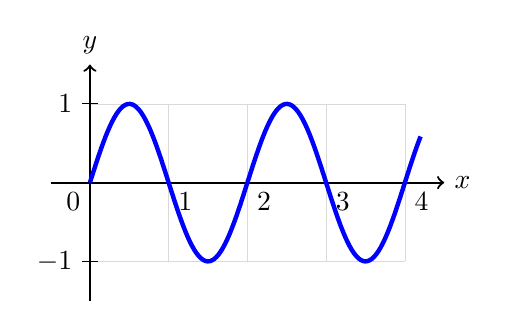
\begin{tikzpicture}[scale=1]
    % Grid
    \draw[help lines, gray!30] (0,-1) grid (4,1);
    
    % Axes
    \draw[->, thick] (-0.5,0) -- (4.5,0) node[right] {$x$};
    \draw[->, thick] (0,-1.5) -- (0,1.5) node[above] {$y$};
    
    % Function y = sin(pi*x)
    \draw[ultra thick, blue, domain=0:4.2, samples=150] plot (\x, {sin(\x*180)});
    
    % Labels
    \node[below left] at (0,0) {$0$};
    \foreach \x in {1,2,3,4} \node[below right] at (\x,0) {$\x$};
    \draw (0.1, 1) -- (-0.1, 1) node[left] {$1$};
    \draw (0.1, -1) -- (-0.1, -1) node[left] {$-1$};
\end{tikzpicture}
